\section{Introduction}
\label{sec:introduction}

% state the learning objective 
The objective of this laboratory assignment is to study the circuit that can be seen in Figure~\ref{fig:T2Circuit}.
 
The circuit is composed by eleven components. These include an independent sinusoidal voltage source, a current-controlled voltage source, one current source (voltage-controlled), seven resistors and one capacitor.
The indepedent source's behaviour is showcased in the following equation:
\begin {equation}
   v_s(t)= V_s u(-t) + sin(2\pi f t)u(t)
   \end {equation}
   
 Furthermore, the circuit contains thirteen meshes (four of which are essential) and eight nodes.
The values for the resistors and the the capacitor, as well as the values of the constansts related with the dependent sources and the initial value(corresponding to t<0) of the independent voltage source, are provided by the Python script

In Section~\ref{sec:analysis}, a theoretical analysis of the circuit is
presented. The analysis was divided in 6 different parts, where each of them represented a step in solving the complex problem that was presented. In Section~\ref{sec:simulation}, the circuit is analysed by
simulation, and the results are compared to the theoretical results obtained in Section~\ref{sec:analysis}. In this section, , we  The conclusions of this study are outlined in
Section~\ref{sec:conclusion}.

\vspace{4.0cm}

\begin{figure}[h] \centering
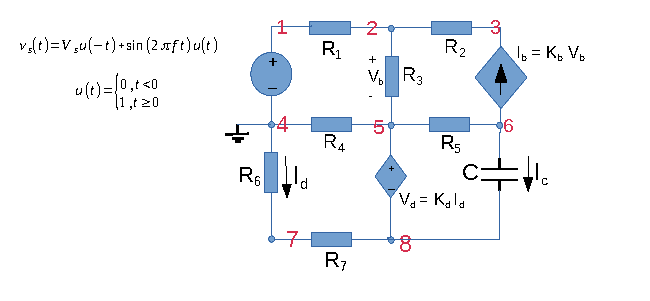
\includegraphics[width=0.8\linewidth]{T2Circuit.pdf}
\caption{Studied circuit.}
\label{fig:T2Circuit}
\end{figure}
